%%
%% Figures for additional distance metric.
%% 

\begin{figure*}
  \centering
  \begin{tabular}{ccc}
    
    \begin{minipage}{2in}
      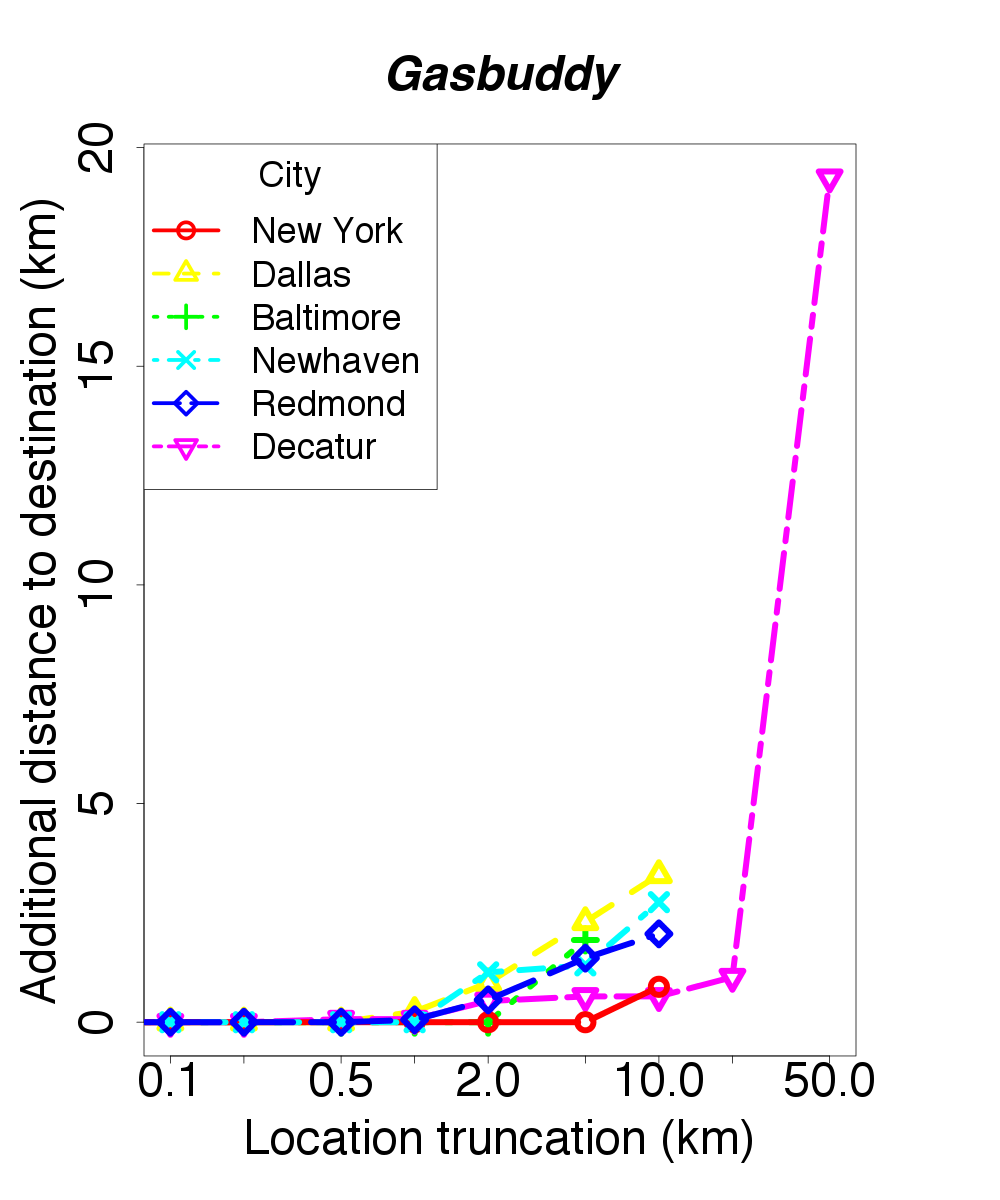
\includegraphics[width=\textwidth]
                      {data/gasbuddy/plots/medians_across_city_additional_distance}
    \end{minipage}
    
    % [width=.6\textwidth]
    \begin{minipage}{2in}
      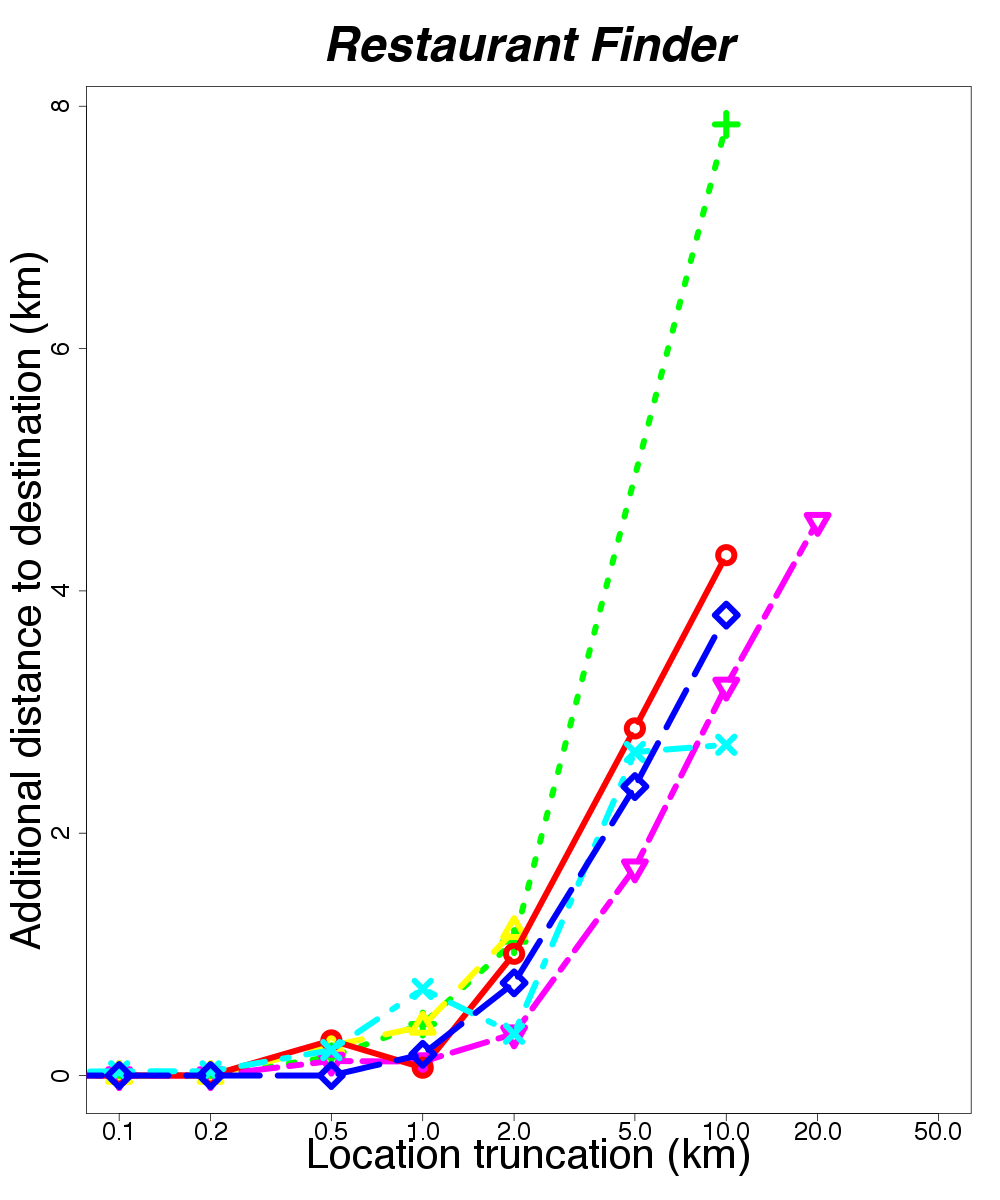
\includegraphics[width=\textwidth]
                      {data/restaurant_finder/plots/medians_across_city_additional_distance}
    \end{minipage}
    
    \begin{minipage}{2in}
      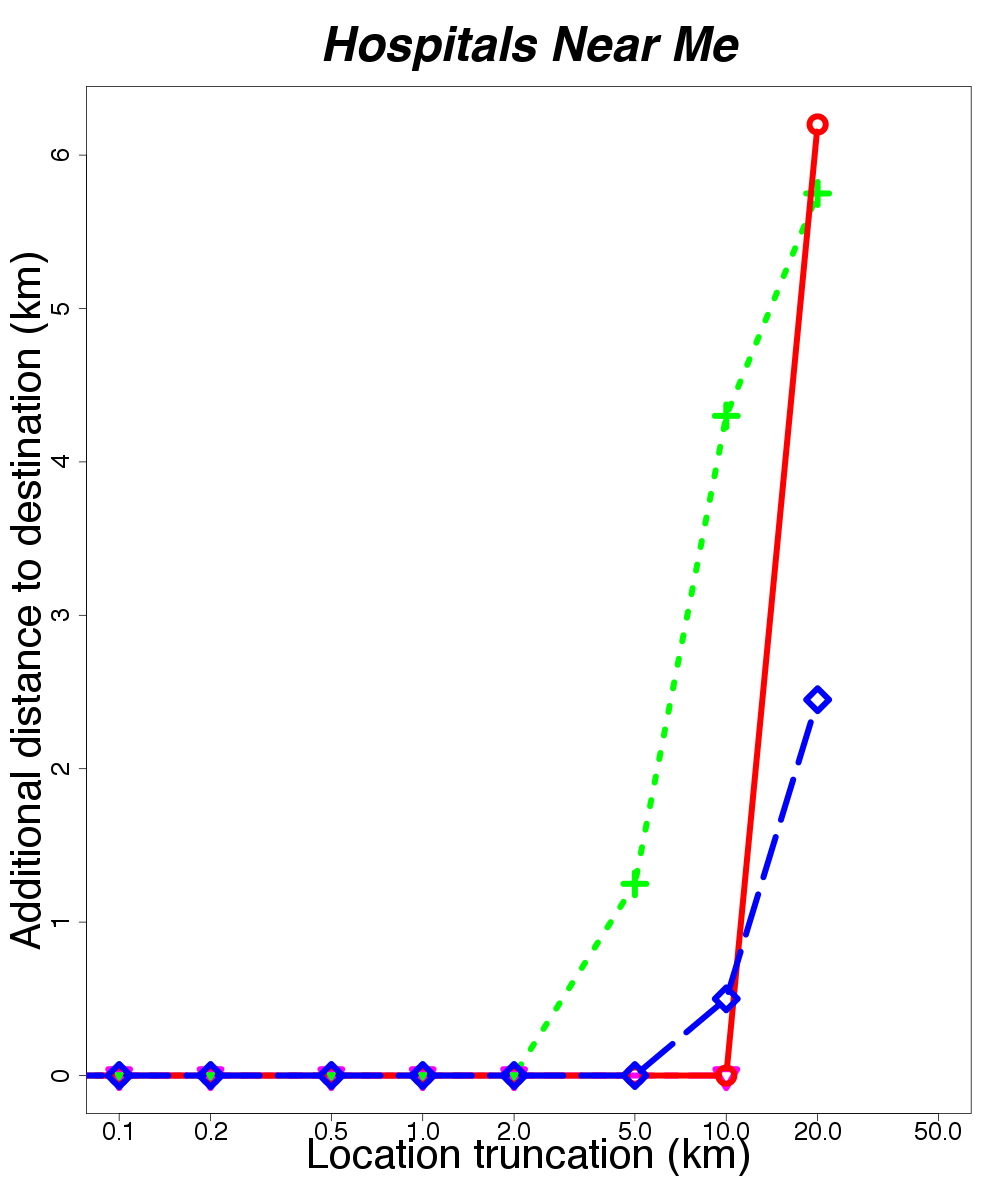
\includegraphics[width=\textwidth]
                      {data/hospitals/plots/medians_across_city_additional_distance}
    \end{minipage}
    
    \\
    \begin{minipage}{2in}
      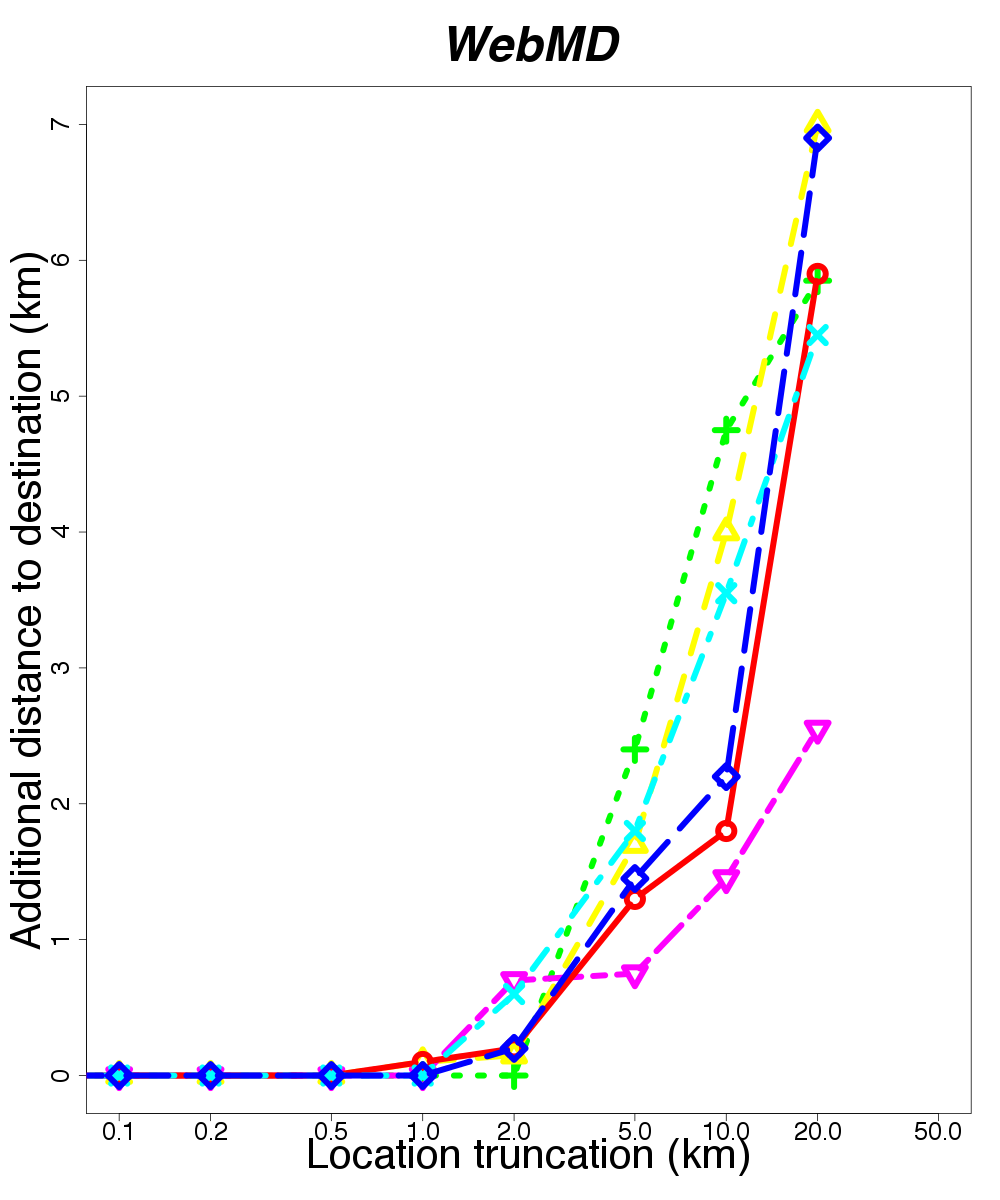
\includegraphics[width=\textwidth]
                      {data/webmd/plots/medians_across_city_additional_distance}
    \end{minipage}
    
    \begin{minipage}{2in}
      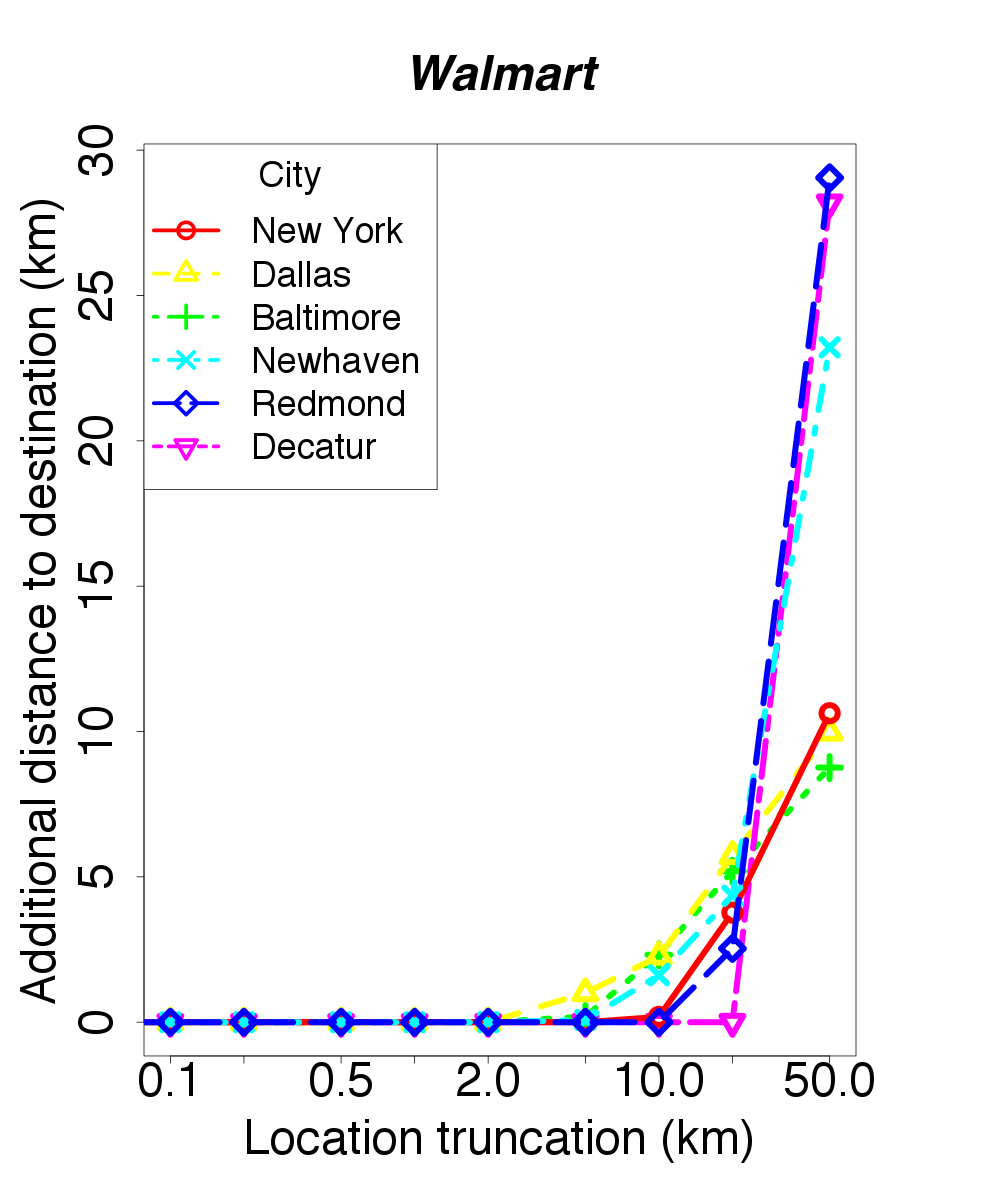
\includegraphics[width=\textwidth]
                      {data/walmart/plots/medians_across_city_additional_distance}
    \end{minipage}
    
    \begin{minipage}{2in}
      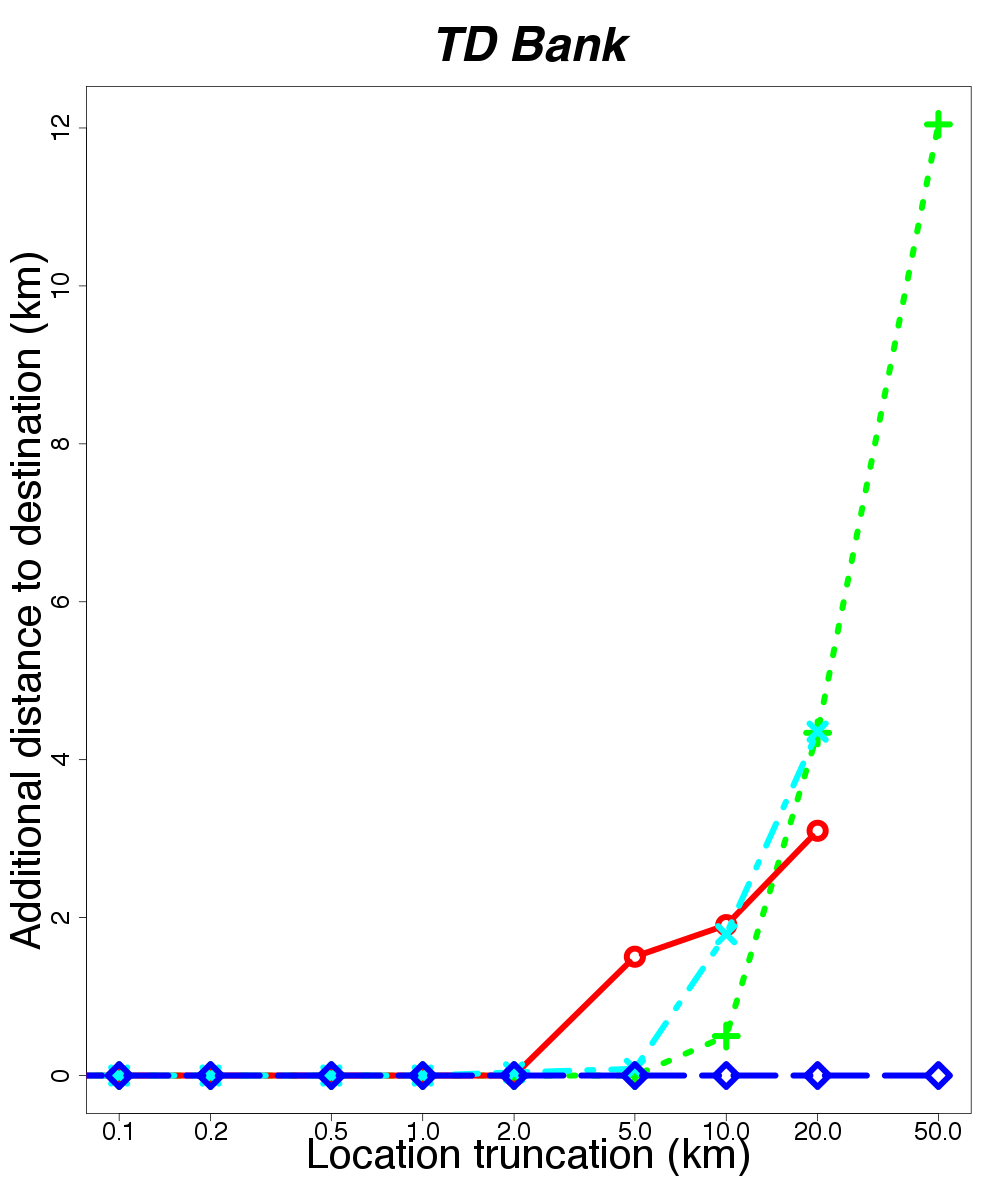
\includegraphics[width=\textwidth]
                      {data/tdbank/plots/medians_across_city_additional_distance}
    \end{minipage}
  \end{tabular}
  \caption{The additional distance metric applied to every app in our
    test corpus.  The vertical axis indicates the additional distance
    a user would have to travel if they went to the top result in the
    nominal output, versus the reference output.}
  \label{fig:add_distance}
\end{figure*}

